%!TEX root = proj.tex

\section{Normalization of travel demand}
As etablished by the descriptive analysis of travel demand data in \Cref{ch:desc_traveldemand}, the expected demand varies throughout the time of the day, and the day of the week. In order to find any impacts of weather we must focus on deviations from the normal and expected pattern.

Once we have presented our models, we want to evaluate them using the following measures: \emph{mean absolute percentage error} (MAPE) and \emph{root mean square error} (RMSE) cf.~\Cref{eq:mape,eq:rmse}.
\vspace{-2em}
\begin{multicols}{2}
\begin{equation}
    \textrm{MAPE}(D, \widehat{D}) = \frac{1}{n} \sum_{i = 1}^{n} \left| \frac{\gls{D_i} - \gls{D_i_pred}}{\gls{D_i}} \right| 
    \label{eq:mape} 
\end{equation}
\break
\vspace{-6.5pt}
\begin{equation}
    \textrm{RMSE}(D, \widehat{D}) = \sqrt{\frac{\sum_{i = 1}^{n} \gls{D_i} - \gls{D_i_pred}}{n}}
    \label{eq:rmse}
\end{equation}
\end{multicols}

\subsection{Modeling with single LR-model}
The initial approach for this is to fit a \emph{single} linear regression (LR) model, $\mathcal{M}_\star$ on the \emph{entire} travel demand data, using time of the day, \gls{hour_i}, day of the week, \gls{dow_i}, their interaction, along with the overall day measure, \gls{day_i}, as shown in~(\ref{eq:fit}). The intuition about this approach is to let the model capture as much as possible of the travel demand variation that can be explained by the observations being measured at different times. The last term, \gls{day_i}, allows for the capture of an overall increase/decline of travel demand. 
\begin{equation}
    \mathcal{M}_\star \models \sqrt[\leftroot{0}\uproot{2}4]{\textit{\gls{D_i}}} \sim \gls{dow_i} + \gls{hour_i} + \gls{dow_i}:\gls{hour_i} + \gls{day_i}  
    \label{eq:fit}
\end{equation}

Notice that we transform the response to the fourth root of the travel demand. This is to ensure homoscedasticity of error. We verify that model assumptions hold using \Cref{fit-assumptions}. From the \emph{Residuals vs Fitted}-plot we see linear behavior, and normal error is also acceptable cf. \emph{Normal Q-Q}-plot. Constant variance of error is also confirmed by the uniform spread in the \emph{Scale-Location}-plot. Finally we might identify some outliers in the \emph{Residuals vs Fitted}-plot, but as outliers is part of what we are trying to identify (e.g.\ any non-normal travel demand), we will not remove any of them. Finally we confirm that all terms are contributing statistically significant to the model, i.e.\ no non-significant terms can be dropped from the model.

\begin{figure}[!p]
    \center
    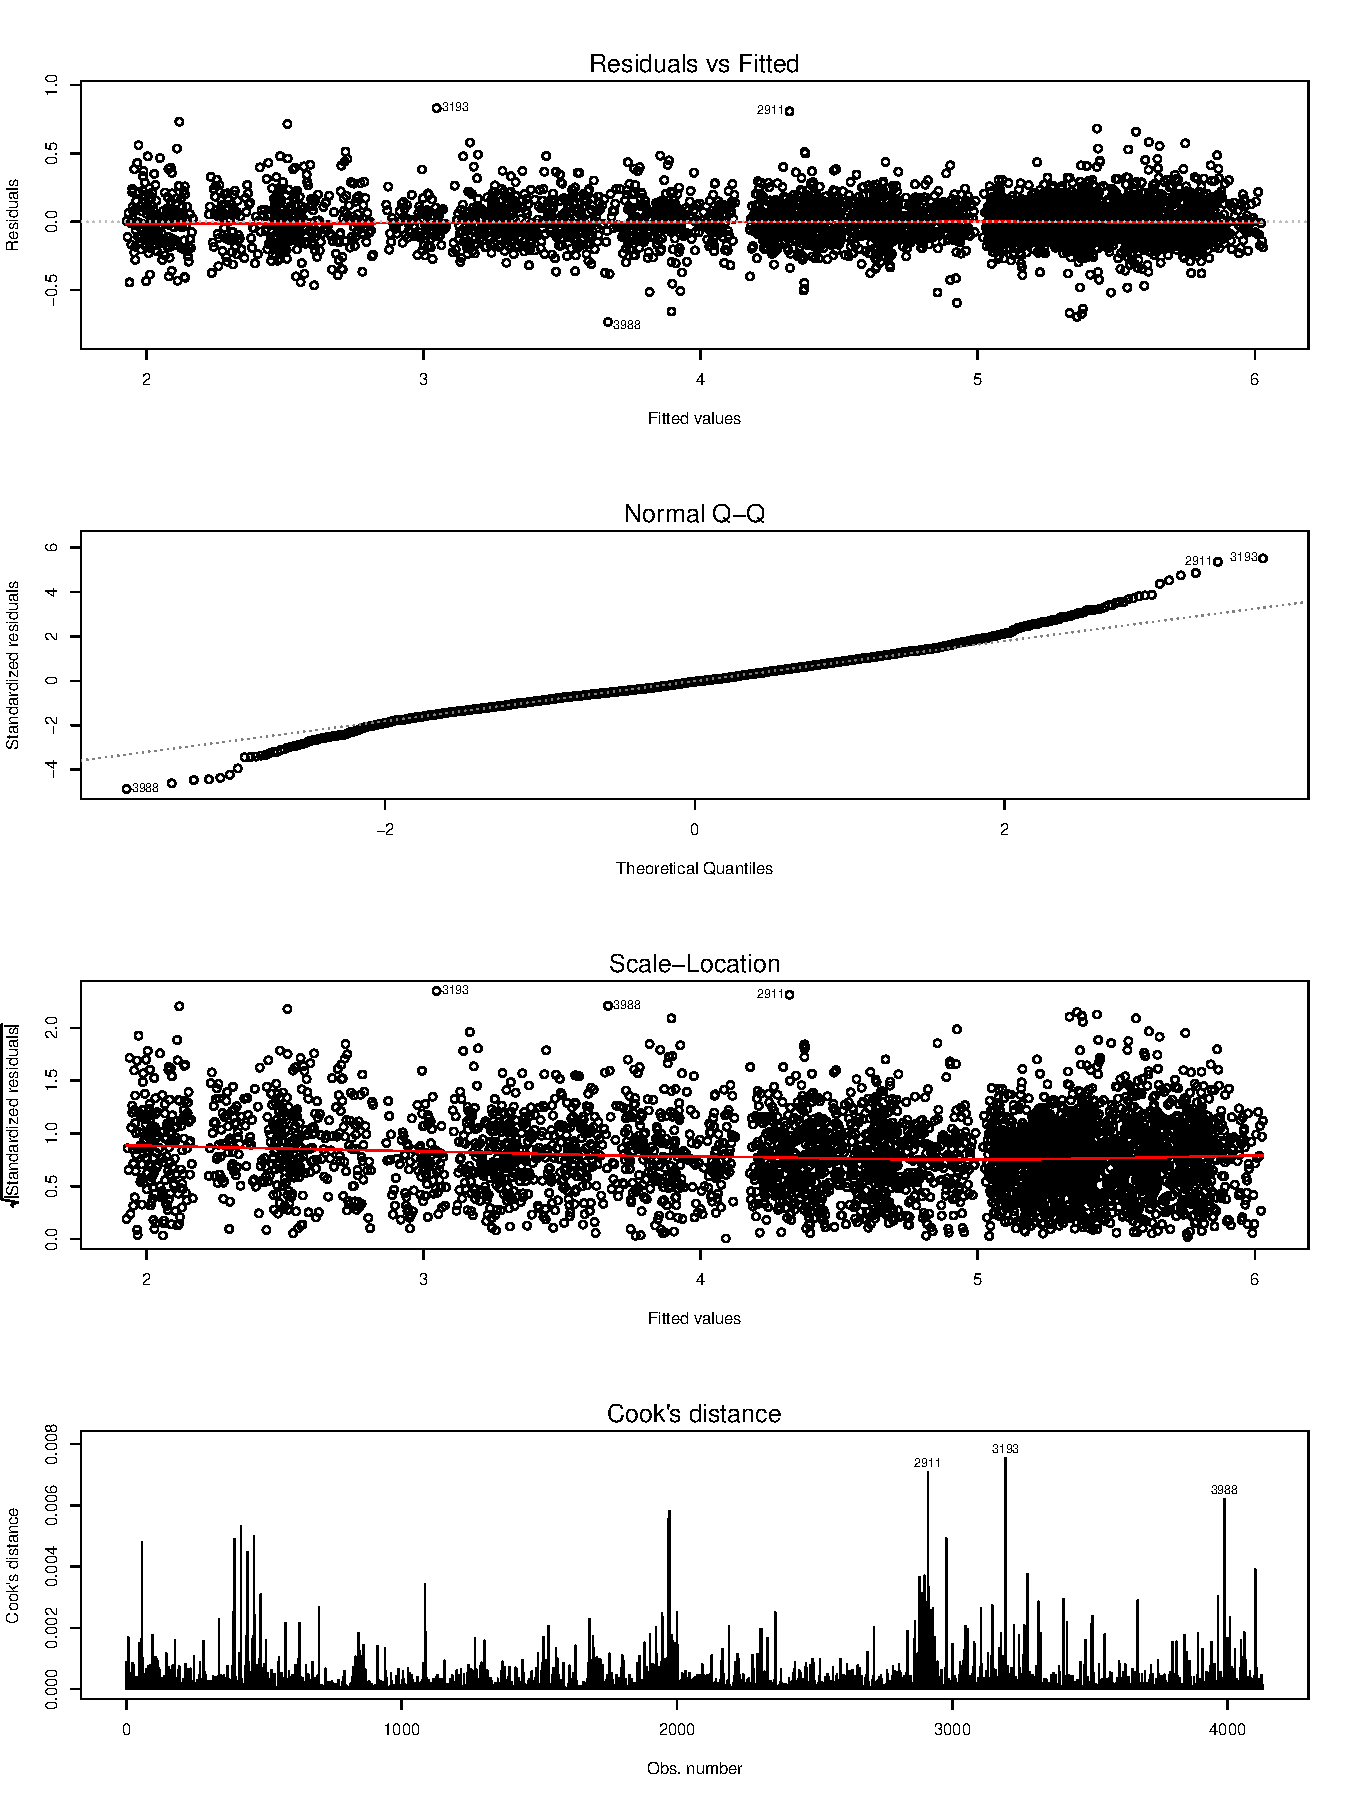
\includegraphics[width=\textwidth]{../plots/fit-assumptions}    
    \caption{Plots for confirming model assumptions.}    
    \label{fit-assumptions}
\end{figure}

With model assumptions checked, the model is evaluated cf.\ \Cref{tab:model_star_eval}. It is seen that the model captures quite well on the surface, with an overall MAPE of 12\% and RMSE of\ $~70$~passengers. There are however large deviations in the  of the different {day types}, \gls{daytype_i}, and {peek classes}, \gls{peek_i}.
\begin{table}[!ht]
    \center
    \begin{tabular}{llrr}
 $\mathit{dt}$ & $\mathit{peek}$ & RMSE & MAPE \\ 
  \hline
\hline
Weekend & No Peek & 60.15 & 10.4\% \\ 
   \hline
Weekday & No Peek & 55.46 & 13.1\% \\ 
   \hline
Weekday & Morning & 140.07 & 10.7\% \\ 
   \hline
Weekday & Afternoon & 111.12 & 7.8\% \\ 
   \hline
\hline
Overall &  & 71.11 & 11.7\% \\ 
  \end{tabular}

    \caption{Evaluation of initial model approach.}
    \label{tab:model_star_eval}
\end{table}

\subsection{Modeling using multiple independent models}
Different configurations of independent sub-models is investigated by dividing the travel demand data set based on \gls{daytype_i} and \gls{peek_i}, and the combination of both. It is found that the best results are achieved by segmenting by \gls{peek_i}. Based on this three models are defined cf.\ \Cref{eq:model_np,eq:model_mp,eq:model_ap}. Notice that model-selection revealed that the interaction-term $\gls{dow_i}:\gls{hour_i}$ is not significant for $\mathcal{M}_{\textsc{Morning}}$, and has thus been dropped from the model.
\begin{align}
\mathcal{M}_{\textsc{No}} &\models \sqrt[\leftroot{0}\uproot{2}4]{\textit{\gls{D_i}}} \sim \gls{dow_i} + \gls{hour_i} + \gls{dow_i}:\gls{hour_i} + \gls{day_i} &\text{for} \; \gls{peek_i} = \textsc{No} \label{eq:model_np} \\
\mathcal{M}_{\textsc{Morning}} &\models \sqrt[\leftroot{0}\uproot{2}4]{\textit{\gls{D_i}}} \sim \gls{dow_i} + \gls{hour_i} + \gls{day_i}  &\text{for} \; \gls
{peek_i} = \textsc{Morning}  \label{eq:model_mp} \\
\mathcal{M}_{\textsc{Afternoon}} &\models \sqrt[\leftroot{0}\uproot{2}4]{\textit{\gls{D_i}}} \sim \gls{dow_i} + \gls{hour_i} + \gls{dow_i}:\gls{hour_i} + \gls{day_i}  &\text{for} \; \gls{peek_i} = \textsc{Afternoon}  \label{eq:model_ap}
\end{align}

Once again model assumptions are checked using plots (See~\Cref{appx:model_assumptions}) and are accepted, although the acceptance of normal errors is weak for $\mathcal{M}_{\textsc{Morning}}$. The evaluation result is shown in~\Cref{tab:model_independent_eval}, and while the segmentation does improves the MAPE and RMSE, the improvements are minor. Only $\textsc{Weekday}/\textsc{Morning}$ seems to benefit noticeably, while RMSE for $\textsc{Weekday}/\textsc{No Peek}$ actually sees a minimal decline.
\begin{table}[!ht]
    \center
    \begin{tabular}{llrr}
 $\mathit{dt}$ & $\mathit{peek}$ & RMSE & MAPE \\ 
  \hline
\hline
Weekend & No Peek & 59.80 & 10.3\% \\ 
   \hline
Weekday & No Peek & 55.64 & 13.1\% \\ 
   \hline
Weekday & Morning & 136.53 & 10.6\% \\ 
   \hline
Weekday & Afternoon & 109.70 & 7.6\% \\ 
   \hline
\hline
Overall &  & 70.49 & 11.7\% \\ 
  \end{tabular}

    \caption{Evaluation of multiple independent models approach.}
    \label{tab:model_independent_eval}
\end{table}

\subsection{Model application}
The model is then applied to the data, yielding the estimated travel demand~\gls{D_i_pred}, as illustrated in the example in \Cref{fig:travelcard_pred}, which simply shows the first whole week in the data set (``Monday, October 3, 2016''--``Sunday, October 9, 2016'').
\begin{figure}[!ht]
    \center
    % !TEX encoding = UTF-8 Unicode
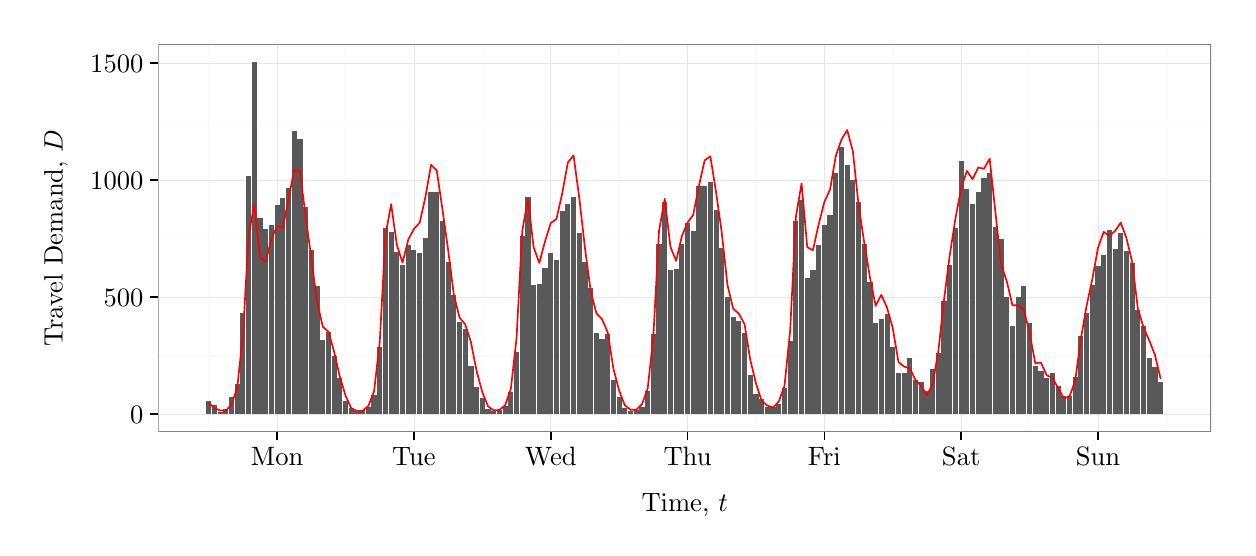
\begin{tikzpicture}[x=1pt,y=1pt]
\definecolor{fillColor}{RGB}{255,255,255}
\path[use as bounding box,fill=fillColor,fill opacity=0.00] (0,0) rectangle (433.62,180.67);
\begin{scope}
\path[clip] (  0.00,  0.00) rectangle (433.62,180.67);
\definecolor{drawColor}{RGB}{255,255,255}
\definecolor{fillColor}{RGB}{255,255,255}

\path[draw=drawColor,line width= 0.6pt,line join=round,line cap=round,fill=fillColor] (  0.00,  0.00) rectangle (433.62,180.68);
\end{scope}
\begin{scope}
\path[clip] ( 47.21, 34.62) rectangle (427.62,174.67);
\definecolor{fillColor}{RGB}{255,255,255}

\path[fill=fillColor] ( 47.21, 34.62) rectangle (427.62,174.67);
\definecolor{drawColor}{gray}{0.98}

\path[draw=drawColor,line width= 0.6pt,line join=round] ( 47.21, 62.14) --
	(427.62, 62.14);

\path[draw=drawColor,line width= 0.6pt,line join=round] ( 47.21,104.44) --
	(427.62,104.44);

\path[draw=drawColor,line width= 0.6pt,line join=round] ( 47.21,146.74) --
	(427.62,146.74);

\path[draw=drawColor,line width= 0.6pt,line join=round] ( 65.43, 34.62) --
	( 65.43,174.67);

\path[draw=drawColor,line width= 0.6pt,line join=round] (114.86, 34.62) --
	(114.86,174.67);

\path[draw=drawColor,line width= 0.6pt,line join=round] (164.29, 34.62) --
	(164.29,174.67);

\path[draw=drawColor,line width= 0.6pt,line join=round] (213.73, 34.62) --
	(213.73,174.67);

\path[draw=drawColor,line width= 0.6pt,line join=round] (263.16, 34.62) --
	(263.16,174.67);

\path[draw=drawColor,line width= 0.6pt,line join=round] (312.59, 34.62) --
	(312.59,174.67);

\path[draw=drawColor,line width= 0.6pt,line join=round] (362.03, 34.62) --
	(362.03,174.67);

\path[draw=drawColor,line width= 0.6pt,line join=round] (411.46, 34.62) --
	(411.46,174.67);
\definecolor{drawColor}{gray}{0.90}

\path[draw=drawColor,line width= 0.2pt,line join=round] ( 47.21, 40.99) --
	(427.62, 40.99);

\path[draw=drawColor,line width= 0.2pt,line join=round] ( 47.21, 83.29) --
	(427.62, 83.29);

\path[draw=drawColor,line width= 0.2pt,line join=round] ( 47.21,125.59) --
	(427.62,125.59);

\path[draw=drawColor,line width= 0.2pt,line join=round] ( 47.21,167.89) --
	(427.62,167.89);

\path[draw=drawColor,line width= 0.2pt,line join=round] ( 90.14, 34.62) --
	( 90.14,174.67);

\path[draw=drawColor,line width= 0.2pt,line join=round] (139.58, 34.62) --
	(139.58,174.67);

\path[draw=drawColor,line width= 0.2pt,line join=round] (189.01, 34.62) --
	(189.01,174.67);

\path[draw=drawColor,line width= 0.2pt,line join=round] (238.44, 34.62) --
	(238.44,174.67);

\path[draw=drawColor,line width= 0.2pt,line join=round] (287.88, 34.62) --
	(287.88,174.67);

\path[draw=drawColor,line width= 0.2pt,line join=round] (337.31, 34.62) --
	(337.31,174.67);

\path[draw=drawColor,line width= 0.2pt,line join=round] (386.74, 34.62) --
	(386.74,174.67);
\definecolor{fillColor}{gray}{0.35}

\path[fill=fillColor] ( 64.50, 40.99) rectangle ( 66.35, 45.81);

\path[fill=fillColor] ( 66.56, 40.99) rectangle ( 68.41, 44.20);

\path[fill=fillColor] ( 68.62, 40.99) rectangle ( 70.47, 41.92);

\path[fill=fillColor] ( 70.68, 40.99) rectangle ( 72.53, 42.94);

\path[fill=fillColor] ( 72.74, 40.99) rectangle ( 74.59, 47.08);

\path[fill=fillColor] ( 74.80, 40.99) rectangle ( 76.65, 51.99);

\path[fill=fillColor] ( 76.86, 40.99) rectangle ( 78.71, 77.54);

\path[fill=fillColor] ( 78.92, 40.99) rectangle ( 80.77,127.03);

\path[fill=fillColor] ( 80.98, 40.99) rectangle ( 82.83,168.31);

\path[fill=fillColor] ( 83.04, 40.99) rectangle ( 84.89,111.88);

\path[fill=fillColor] ( 85.10, 40.99) rectangle ( 86.95,107.82);

\path[fill=fillColor] ( 87.16, 40.99) rectangle ( 89.01,109.43);

\path[fill=fillColor] ( 89.22, 40.99) rectangle ( 91.07,116.70);

\path[fill=fillColor] ( 91.28, 40.99) rectangle ( 93.13,119.07);

\path[fill=fillColor] ( 93.33, 40.99) rectangle ( 95.19,122.71);

\path[fill=fillColor] ( 95.39, 40.99) rectangle ( 97.25,143.27);

\path[fill=fillColor] ( 97.45, 40.99) rectangle ( 99.31,140.56);

\path[fill=fillColor] ( 99.51, 40.99) rectangle (101.37,116.03);

\path[fill=fillColor] (101.57, 40.99) rectangle (103.43,100.21);

\path[fill=fillColor] (103.63, 40.99) rectangle (105.49, 87.26);

\path[fill=fillColor] (105.69, 40.99) rectangle (107.55, 67.72);

\path[fill=fillColor] (107.75, 40.99) rectangle (109.61, 70.77);

\path[fill=fillColor] (109.81, 40.99) rectangle (111.67, 62.14);

\path[fill=fillColor] (111.87, 40.99) rectangle (113.73, 54.10);

\path[fill=fillColor] (113.93, 40.99) rectangle (115.79, 45.73);

\path[fill=fillColor] (115.99, 40.99) rectangle (117.85, 43.27);

\path[fill=fillColor] (118.05, 40.99) rectangle (119.91, 42.17);

\path[fill=fillColor] (120.11, 40.99) rectangle (121.97, 42.51);

\path[fill=fillColor] (122.17, 40.99) rectangle (124.03, 43.70);

\path[fill=fillColor] (124.23, 40.99) rectangle (126.08, 47.84);

\path[fill=fillColor] (126.29, 40.99) rectangle (128.14, 65.35);

\path[fill=fillColor] (128.35, 40.99) rectangle (130.20,108.24);

\path[fill=fillColor] (130.41, 40.99) rectangle (132.26,106.89);

\path[fill=fillColor] (132.47, 40.99) rectangle (134.32, 99.78);

\path[fill=fillColor] (134.53, 40.99) rectangle (136.38, 95.05);

\path[fill=fillColor] (136.59, 40.99) rectangle (138.44,102.07);

\path[fill=fillColor] (138.65, 40.99) rectangle (140.50,100.21);

\path[fill=fillColor] (140.71, 40.99) rectangle (142.56, 99.28);

\path[fill=fillColor] (142.77, 40.99) rectangle (144.62,104.78);

\path[fill=fillColor] (144.83, 40.99) rectangle (146.68,121.44);

\path[fill=fillColor] (146.89, 40.99) rectangle (148.74,121.36);

\path[fill=fillColor] (148.95, 40.99) rectangle (150.80,110.78);

\path[fill=fillColor] (151.01, 40.99) rectangle (152.86, 95.89);

\path[fill=fillColor] (153.07, 40.99) rectangle (154.92, 84.13);

\path[fill=fillColor] (155.13, 40.99) rectangle (156.98, 74.32);

\path[fill=fillColor] (157.19, 40.99) rectangle (159.04, 71.95);

\path[fill=fillColor] (159.25, 40.99) rectangle (161.10, 58.25);

\path[fill=fillColor] (161.31, 40.99) rectangle (163.16, 50.89);

\path[fill=fillColor] (163.37, 40.99) rectangle (165.22, 46.83);

\path[fill=fillColor] (165.43, 40.99) rectangle (167.28, 42.85);

\path[fill=fillColor] (167.49, 40.99) rectangle (169.34, 42.00);

\path[fill=fillColor] (169.55, 40.99) rectangle (171.40, 42.43);

\path[fill=fillColor] (171.61, 40.99) rectangle (173.46, 43.95);

\path[fill=fillColor] (173.66, 40.99) rectangle (175.52, 49.03);

\path[fill=fillColor] (175.72, 40.99) rectangle (177.58, 63.32);

\path[fill=fillColor] (177.78, 40.99) rectangle (179.64,105.45);

\path[fill=fillColor] (179.84, 40.99) rectangle (181.70,119.58);

\path[fill=fillColor] (181.90, 40.99) rectangle (183.76, 87.86);

\path[fill=fillColor] (183.96, 40.99) rectangle (185.82, 87.94);

\path[fill=fillColor] (186.02, 40.99) rectangle (187.88, 93.86);

\path[fill=fillColor] (188.08, 40.99) rectangle (189.94, 99.36);

\path[fill=fillColor] (190.14, 40.99) rectangle (192.00, 96.74);

\path[fill=fillColor] (192.20, 40.99) rectangle (194.06,114.59);

\path[fill=fillColor] (194.26, 40.99) rectangle (196.12,117.13);

\path[fill=fillColor] (196.32, 40.99) rectangle (198.18,119.33);

\path[fill=fillColor] (198.38, 40.99) rectangle (200.24,106.38);

\path[fill=fillColor] (200.44, 40.99) rectangle (202.30, 95.89);

\path[fill=fillColor] (202.50, 40.99) rectangle (204.35, 86.59);

\path[fill=fillColor] (204.56, 40.99) rectangle (206.41, 70.34);

\path[fill=fillColor] (206.62, 40.99) rectangle (208.47, 68.15);

\path[fill=fillColor] (208.68, 40.99) rectangle (210.53, 70.09);

\path[fill=fillColor] (210.74, 40.99) rectangle (212.59, 53.51);

\path[fill=fillColor] (212.80, 40.99) rectangle (214.65, 47.17);

\path[fill=fillColor] (214.86, 40.99) rectangle (216.71, 43.27);

\path[fill=fillColor] (216.92, 40.99) rectangle (218.77, 42.17);

\path[fill=fillColor] (218.98, 40.99) rectangle (220.83, 42.51);

\path[fill=fillColor] (221.04, 40.99) rectangle (222.89, 43.78);

\path[fill=fillColor] (223.10, 40.99) rectangle (224.95, 49.28);

\path[fill=fillColor] (225.16, 40.99) rectangle (227.01, 69.92);

\path[fill=fillColor] (227.22, 40.99) rectangle (229.07,102.66);

\path[fill=fillColor] (229.28, 40.99) rectangle (231.13,117.64);

\path[fill=fillColor] (231.34, 40.99) rectangle (233.19, 93.02);

\path[fill=fillColor] (233.40, 40.99) rectangle (235.25, 93.36);

\path[fill=fillColor] (235.46, 40.99) rectangle (237.31,102.66);

\path[fill=fillColor] (237.52, 40.99) rectangle (239.37,110.11);

\path[fill=fillColor] (239.58, 40.99) rectangle (241.43,107.31);

\path[fill=fillColor] (241.64, 40.99) rectangle (243.49,123.30);

\path[fill=fillColor] (243.70, 40.99) rectangle (245.55,123.30);

\path[fill=fillColor] (245.76, 40.99) rectangle (247.61,124.91);

\path[fill=fillColor] (247.82, 40.99) rectangle (249.67,114.76);

\path[fill=fillColor] (249.88, 40.99) rectangle (251.73,101.05);

\path[fill=fillColor] (251.93, 40.99) rectangle (253.79, 83.20);

\path[fill=fillColor] (253.99, 40.99) rectangle (255.85, 76.01);

\path[fill=fillColor] (256.05, 40.99) rectangle (257.91, 74.66);

\path[fill=fillColor] (258.11, 40.99) rectangle (259.97, 70.51);

\path[fill=fillColor] (260.17, 40.99) rectangle (262.03, 55.20);

\path[fill=fillColor] (262.23, 40.99) rectangle (264.09, 48.43);

\path[fill=fillColor] (264.29, 40.99) rectangle (266.15, 46.57);

\path[fill=fillColor] (266.35, 40.99) rectangle (268.21, 43.70);

\path[fill=fillColor] (268.41, 40.99) rectangle (270.27, 43.70);

\path[fill=fillColor] (270.47, 40.99) rectangle (272.33, 44.54);

\path[fill=fillColor] (272.53, 40.99) rectangle (274.39, 50.63);

\path[fill=fillColor] (274.59, 40.99) rectangle (276.45, 67.55);

\path[fill=fillColor] (276.65, 40.99) rectangle (278.51,110.78);

\path[fill=fillColor] (278.71, 40.99) rectangle (280.57,118.31);

\path[fill=fillColor] (280.77, 40.99) rectangle (282.62, 90.23);

\path[fill=fillColor] (282.83, 40.99) rectangle (284.68, 93.10);

\path[fill=fillColor] (284.89, 40.99) rectangle (286.74,102.24);

\path[fill=fillColor] (286.95, 40.99) rectangle (288.80,109.51);

\path[fill=fillColor] (289.01, 40.99) rectangle (290.86,112.81);

\path[fill=fillColor] (291.07, 40.99) rectangle (292.92,128.04);

\path[fill=fillColor] (293.13, 40.99) rectangle (294.98,137.60);

\path[fill=fillColor] (295.19, 40.99) rectangle (297.04,131.09);

\path[fill=fillColor] (297.25, 40.99) rectangle (299.10,125.76);

\path[fill=fillColor] (299.31, 40.99) rectangle (301.16,117.64);

\path[fill=fillColor] (301.37, 40.99) rectangle (303.22,102.32);

\path[fill=fillColor] (303.43, 40.99) rectangle (305.28, 88.62);

\path[fill=fillColor] (305.49, 40.99) rectangle (307.34, 73.81);

\path[fill=fillColor] (307.55, 40.99) rectangle (309.40, 75.34);

\path[fill=fillColor] (309.61, 40.99) rectangle (311.46, 77.28);

\path[fill=fillColor] (311.67, 40.99) rectangle (313.52, 65.10);

\path[fill=fillColor] (313.73, 40.99) rectangle (315.58, 55.88);

\path[fill=fillColor] (315.79, 40.99) rectangle (317.64, 55.71);

\path[fill=fillColor] (317.85, 40.99) rectangle (319.70, 61.21);

\path[fill=fillColor] (319.91, 40.99) rectangle (321.76, 53.43);

\path[fill=fillColor] (321.97, 40.99) rectangle (323.82, 52.66);

\path[fill=fillColor] (324.03, 40.99) rectangle (325.88, 49.53);

\path[fill=fillColor] (326.09, 40.99) rectangle (327.94, 57.32);

\path[fill=fillColor] (328.15, 40.99) rectangle (330.00, 63.15);

\path[fill=fillColor] (330.20, 40.99) rectangle (332.06, 81.77);

\path[fill=fillColor] (332.26, 40.99) rectangle (334.12, 94.79);

\path[fill=fillColor] (334.32, 40.99) rectangle (336.18,108.16);

\path[fill=fillColor] (336.38, 40.99) rectangle (338.24,132.52);

\path[fill=fillColor] (338.44, 40.99) rectangle (340.30,122.54);

\path[fill=fillColor] (340.50, 40.99) rectangle (342.36,116.87);

\path[fill=fillColor] (342.56, 40.99) rectangle (344.42,121.19);

\path[fill=fillColor] (344.62, 40.99) rectangle (346.48,126.26);

\path[fill=fillColor] (346.68, 40.99) rectangle (348.54,128.13);

\path[fill=fillColor] (348.74, 40.99) rectangle (350.60,108.50);

\path[fill=fillColor] (350.80, 40.99) rectangle (352.66,104.18);

\path[fill=fillColor] (352.86, 40.99) rectangle (354.72, 83.29);

\path[fill=fillColor] (354.92, 40.99) rectangle (356.78, 72.71);

\path[fill=fillColor] (356.98, 40.99) rectangle (358.84, 83.29);

\path[fill=fillColor] (359.04, 40.99) rectangle (360.89, 87.43);

\path[fill=fillColor] (361.10, 40.99) rectangle (362.95, 73.98);

\path[fill=fillColor] (363.16, 40.99) rectangle (365.01, 58.25);

\path[fill=fillColor] (365.22, 40.99) rectangle (367.07, 56.56);

\path[fill=fillColor] (367.28, 40.99) rectangle (369.13, 54.19);

\path[fill=fillColor] (369.34, 40.99) rectangle (371.19, 55.96);

\path[fill=fillColor] (371.40, 40.99) rectangle (373.25, 51.14);

\path[fill=fillColor] (373.46, 40.99) rectangle (375.31, 47.42);

\path[fill=fillColor] (375.52, 40.99) rectangle (377.37, 47.42);

\path[fill=fillColor] (377.58, 40.99) rectangle (379.43, 54.36);

\path[fill=fillColor] (379.64, 40.99) rectangle (381.49, 69.33);

\path[fill=fillColor] (381.70, 40.99) rectangle (383.55, 77.54);

\path[fill=fillColor] (383.76, 40.99) rectangle (385.61, 87.69);

\path[fill=fillColor] (385.82, 40.99) rectangle (387.67, 94.46);

\path[fill=fillColor] (387.88, 40.99) rectangle (389.73, 98.69);

\path[fill=fillColor] (389.94, 40.99) rectangle (391.79,107.48);

\path[fill=fillColor] (392.00, 40.99) rectangle (393.85,100.80);

\path[fill=fillColor] (394.06, 40.99) rectangle (395.91,106.38);

\path[fill=fillColor] (396.12, 40.99) rectangle (397.97,100.04);

\path[fill=fillColor] (398.18, 40.99) rectangle (400.03, 95.64);

\path[fill=fillColor] (400.24, 40.99) rectangle (402.09, 78.64);

\path[fill=fillColor] (402.30, 40.99) rectangle (404.15, 72.80);

\path[fill=fillColor] (404.36, 40.99) rectangle (406.21, 61.29);

\path[fill=fillColor] (406.42, 40.99) rectangle (408.27, 58.08);

\path[fill=fillColor] (408.47, 40.99) rectangle (410.33, 52.75);
\definecolor{drawColor}{RGB}{255,0,0}

\path[draw=drawColor,line width= 0.6pt,line join=round] ( 65.43, 45.16) --
	( 67.49, 43.17) --
	( 69.55, 42.36) --
	( 71.60, 42.24) --
	( 73.66, 44.51) --
	( 75.72, 50.58) --
	( 77.78, 69.58) --
	( 79.84,105.62) --
	( 81.90,116.95) --
	( 83.96, 97.58) --
	( 86.02, 96.14) --
	( 88.08,104.36) --
	( 90.14,109.00) --
	( 92.20,108.30) --
	( 94.26,118.80) --
	( 96.32,129.23) --
	( 98.38,128.74) --
	(100.44,112.31) --
	(102.50, 97.41) --
	(104.56, 81.64) --
	(106.62, 72.64) --
	(108.68, 70.81) --
	(110.74, 63.52) --
	(112.80, 54.50) --
	(114.86, 47.74) --
	(116.92, 43.10) --
	(118.98, 42.18) --
	(121.04, 42.24) --
	(123.10, 43.99) --
	(125.16, 49.19) --
	(127.22, 67.02) --
	(129.28,105.59) --
	(131.34,116.91) --
	(133.40,102.18) --
	(135.46, 95.75) --
	(137.52,104.04) --
	(139.58,107.98) --
	(141.64,110.15) --
	(143.70,119.34) --
	(145.76,131.11) --
	(147.82,129.10) --
	(149.87,115.04) --
	(151.93,100.37) --
	(153.99, 84.23) --
	(156.05, 75.89) --
	(158.11, 73.47) --
	(160.17, 67.03) --
	(162.23, 56.53) --
	(164.29, 48.96) --
	(166.35, 43.85) --
	(168.41, 42.40) --
	(170.47, 42.52) --
	(172.53, 44.20) --
	(174.59, 50.12) --
	(176.65, 68.41) --
	(178.71,107.20) --
	(180.77,118.72) --
	(182.83,101.29) --
	(184.89, 95.66) --
	(186.95,103.48) --
	(189.01,110.05) --
	(191.07,111.52) --
	(193.13,120.60) --
	(195.19,131.95) --
	(197.25,134.51) --
	(199.31,119.28) --
	(201.37,101.05) --
	(203.43, 85.60) --
	(205.49, 77.51) --
	(207.55, 75.34) --
	(209.61, 70.53) --
	(211.67, 57.37) --
	(213.73, 49.52) --
	(215.79, 44.20) --
	(217.85, 42.58) --
	(219.91, 42.61) --
	(221.97, 44.60) --
	(224.03, 50.19) --
	(226.09, 69.07) --
	(228.14,107.29) --
	(230.20,118.83) --
	(232.26,101.50) --
	(234.32, 96.38) --
	(236.38,105.33) --
	(238.44,110.26) --
	(240.50,113.05) --
	(242.56,123.50) --
	(244.62,132.71) --
	(246.68,134.20) --
	(248.74,121.28) --
	(250.80,106.69) --
	(252.86, 87.75) --
	(254.92, 79.14) --
	(256.98, 77.34) --
	(259.04, 73.55) --
	(261.10, 60.66) --
	(263.16, 52.17) --
	(265.22, 45.77) --
	(267.28, 44.11) --
	(269.34, 43.44) --
	(271.40, 45.53) --
	(273.46, 51.18) --
	(275.52, 71.18) --
	(277.58,112.22) --
	(279.64,124.38) --
	(281.70,101.33) --
	(283.76,100.25) --
	(285.82,109.62) --
	(287.88,117.65) --
	(289.94,122.22) --
	(292.00,134.25) --
	(294.06,140.23) --
	(296.12,143.67) --
	(298.18,136.07) --
	(300.24,116.56) --
	(302.30,102.91) --
	(304.36, 90.40) --
	(306.41, 80.20) --
	(308.47, 84.13) --
	(310.53, 79.50) --
	(312.59, 72.13) --
	(314.65, 59.85) --
	(316.71, 58.18) --
	(318.77, 57.58) --
	(320.83, 53.31) --
	(322.89, 51.15) --
	(324.95, 47.91) --
	(327.01, 51.85) --
	(329.07, 63.78) --
	(331.13, 82.43) --
	(333.19, 98.43) --
	(335.25,111.77) --
	(337.31,122.59) --
	(339.37,128.92) --
	(341.43,125.89) --
	(343.49,130.12) --
	(345.55,129.66) --
	(347.61,133.31) --
	(349.67,114.20) --
	(351.73, 95.24) --
	(353.79, 89.05) --
	(355.85, 80.32) --
	(357.91, 80.40) --
	(359.97, 78.72) --
	(362.03, 70.41) --
	(364.09, 59.42) --
	(366.15, 59.64) --
	(368.21, 55.07) --
	(370.27, 54.15) --
	(372.33, 50.53) --
	(374.39, 46.80) --
	(376.45, 47.36) --
	(378.51, 53.02) --
	(380.57, 68.28) --
	(382.63, 80.12) --
	(384.68, 89.66) --
	(386.74,101.06) --
	(388.80,106.88) --
	(390.86,105.36) --
	(392.92,107.22) --
	(394.98,110.23) --
	(397.04,104.65) --
	(399.10, 96.04) --
	(401.16, 79.11) --
	(403.22, 72.33) --
	(405.28, 67.62) --
	(407.34, 62.40) --
	(409.40, 53.73);
\definecolor{drawColor}{gray}{0.50}

\path[draw=drawColor,line width= 0.6pt,line join=round,line cap=round] ( 47.21, 34.62) rectangle (427.62,174.67);
\end{scope}
\begin{scope}
\path[clip] (  0.00,  0.00) rectangle (433.62,180.67);
\definecolor{drawColor}{RGB}{0,0,0}

\node[text=drawColor,anchor=base east,inner sep=0pt, outer sep=0pt, scale=  0.96] at ( 41.81, 37.68) {0};

\node[text=drawColor,anchor=base east,inner sep=0pt, outer sep=0pt, scale=  0.96] at ( 41.81, 79.98) {500};

\node[text=drawColor,anchor=base east,inner sep=0pt, outer sep=0pt, scale=  0.96] at ( 41.81,122.28) {1000};

\node[text=drawColor,anchor=base east,inner sep=0pt, outer sep=0pt, scale=  0.96] at ( 41.81,164.58) {1500};
\end{scope}
\begin{scope}
\path[clip] (  0.00,  0.00) rectangle (433.62,180.67);
\definecolor{drawColor}{RGB}{0,0,0}

\path[draw=drawColor,line width= 0.6pt,line join=round] ( 44.21, 40.99) --
	( 47.21, 40.99);

\path[draw=drawColor,line width= 0.6pt,line join=round] ( 44.21, 83.29) --
	( 47.21, 83.29);

\path[draw=drawColor,line width= 0.6pt,line join=round] ( 44.21,125.59) --
	( 47.21,125.59);

\path[draw=drawColor,line width= 0.6pt,line join=round] ( 44.21,167.89) --
	( 47.21,167.89);
\end{scope}
\begin{scope}
\path[clip] (  0.00,  0.00) rectangle (433.62,180.67);
\definecolor{drawColor}{RGB}{0,0,0}

\path[draw=drawColor,line width= 0.6pt,line join=round] ( 90.14, 31.62) --
	( 90.14, 34.62);

\path[draw=drawColor,line width= 0.6pt,line join=round] (139.58, 31.62) --
	(139.58, 34.62);

\path[draw=drawColor,line width= 0.6pt,line join=round] (189.01, 31.62) --
	(189.01, 34.62);

\path[draw=drawColor,line width= 0.6pt,line join=round] (238.44, 31.62) --
	(238.44, 34.62);

\path[draw=drawColor,line width= 0.6pt,line join=round] (287.88, 31.62) --
	(287.88, 34.62);

\path[draw=drawColor,line width= 0.6pt,line join=round] (337.31, 31.62) --
	(337.31, 34.62);

\path[draw=drawColor,line width= 0.6pt,line join=round] (386.74, 31.62) --
	(386.74, 34.62);
\end{scope}
\begin{scope}
\path[clip] (  0.00,  0.00) rectangle (433.62,180.67);
\definecolor{drawColor}{RGB}{0,0,0}

\node[text=drawColor,anchor=base,inner sep=0pt, outer sep=0pt, scale=  0.96] at ( 90.14, 22.61) {Mon};

\node[text=drawColor,anchor=base,inner sep=0pt, outer sep=0pt, scale=  0.96] at (139.58, 22.61) {Tue};

\node[text=drawColor,anchor=base,inner sep=0pt, outer sep=0pt, scale=  0.96] at (189.01, 22.61) {Wed};

\node[text=drawColor,anchor=base,inner sep=0pt, outer sep=0pt, scale=  0.96] at (238.44, 22.61) {Thu};

\node[text=drawColor,anchor=base,inner sep=0pt, outer sep=0pt, scale=  0.96] at (287.88, 22.61) {Fri};

\node[text=drawColor,anchor=base,inner sep=0pt, outer sep=0pt, scale=  0.96] at (337.31, 22.61) {Sat};

\node[text=drawColor,anchor=base,inner sep=0pt, outer sep=0pt, scale=  0.96] at (386.74, 22.61) {Sun};
\end{scope}
\begin{scope}
\path[clip] (  0.00,  0.00) rectangle (433.62,180.67);
\definecolor{drawColor}{RGB}{0,0,0}

\node[text=drawColor,anchor=base,inner sep=0pt, outer sep=0pt, scale=  0.96] at (237.41,  6.00) {Time, $t$};
\end{scope}
\begin{scope}
\path[clip] (  0.00,  0.00) rectangle (433.62,180.67);
\definecolor{drawColor}{RGB}{0,0,0}

\node[text=drawColor,rotate= 90.00,anchor=base,inner sep=0pt, outer sep=0pt, scale=  0.96] at ( 12.61,104.65) {Travel Demand, $D$};
\end{scope}
\end{tikzpicture}

    \vspace{-1em}
    \caption{Predicted passenger boardings of a single week.}
    \label{fig:travelcard_pred}
\end{figure}

\begin{align}
    \mathit{re}_i &= \frac{D_i - \widehat{D_i}}{\widehat{D_i}}
    \label{eq:error}
\end{align}

From the estimated travel demand, the relative error, \gls{re_i}, is calculated cf.~\Cref{eq:error}. This value can be interpreted as the percentage the $i$'th observation deviates from the expected travel pattern, as explained by the linear regression model.\ I.e.\ a clear positive value of \gls{re_i} indicates \emph{higher} travel demand than the \emph{normal conditions} can explain, and likewise a clear negative value indicates \emph{lower} demand than normal, while values around 0 indicates \emph{normal} behavior.


\Cref{fig:travelcard_error_pct} exemplifies the value of \gls{re_i} on the same subeset of the time series as shown in \Cref{fig:travelcard_pred}, i.e.\ the first whole week in the data set. From the plot it can be \todo{Finish}

\begin{figure}[!ht]
    \center
    % !TEX encoding = UTF-8 Unicode
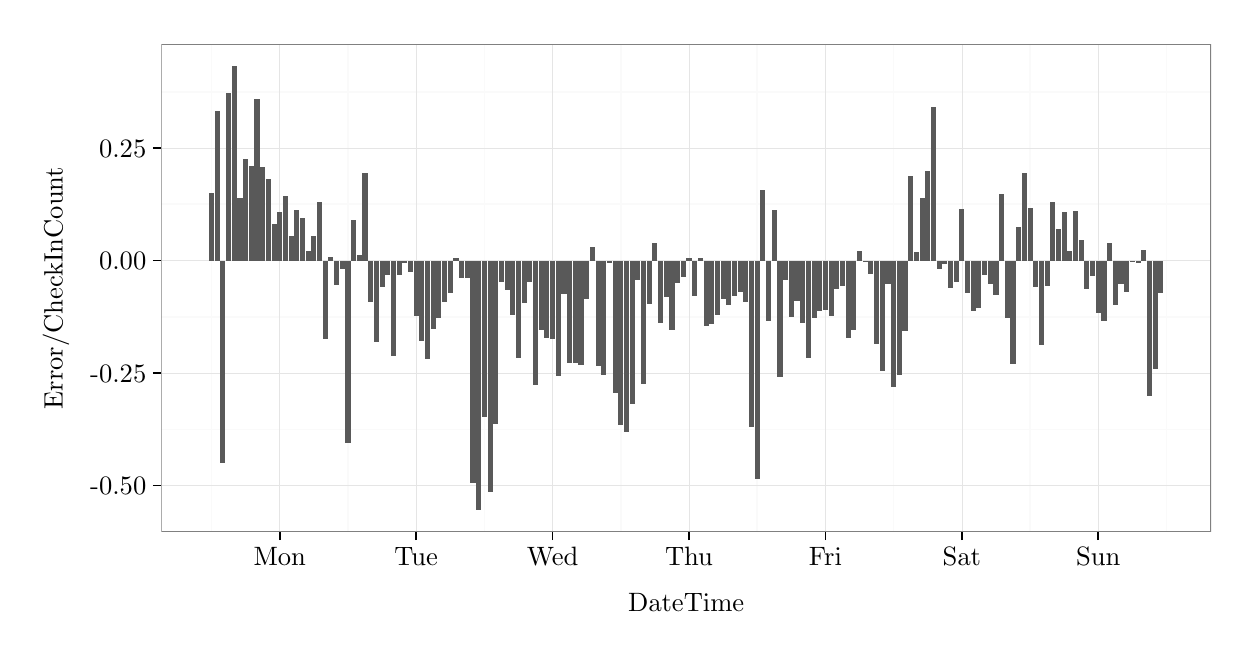
\begin{tikzpicture}[x=1pt,y=1pt]
\definecolor{fillColor}{RGB}{255,255,255}
\path[use as bounding box,fill=fillColor,fill opacity=0.00] (0,0) rectangle (433.62,216.81);
\begin{scope}
\path[clip] (  0.00,  0.00) rectangle (433.62,216.81);
\definecolor{drawColor}{RGB}{255,255,255}
\definecolor{fillColor}{RGB}{255,255,255}

\path[draw=drawColor,line width= 0.6pt,line join=round,line cap=round,fill=fillColor] (  0.00,  0.00) rectangle (433.62,216.81);
\end{scope}
\begin{scope}
\path[clip] ( 48.27, 34.62) rectangle (427.62,210.81);
\definecolor{fillColor}{RGB}{255,255,255}

\path[fill=fillColor] ( 48.27, 34.62) rectangle (427.62,210.81);
\definecolor{drawColor}{gray}{0.98}

\path[draw=drawColor,line width= 0.6pt,line join=round] ( 48.27, 71.65) --
	(427.62, 71.65);

\path[draw=drawColor,line width= 0.6pt,line join=round] ( 48.27,112.32) --
	(427.62,112.32);

\path[draw=drawColor,line width= 0.6pt,line join=round] ( 48.27,152.99) --
	(427.62,152.99);

\path[draw=drawColor,line width= 0.6pt,line join=round] ( 48.27,193.66) --
	(427.62,193.66);

\path[draw=drawColor,line width= 0.6pt,line join=round] ( 66.44, 34.62) --
	( 66.44,210.81);

\path[draw=drawColor,line width= 0.6pt,line join=round] (115.74, 34.62) --
	(115.74,210.81);

\path[draw=drawColor,line width= 0.6pt,line join=round] (165.03, 34.62) --
	(165.03,210.81);

\path[draw=drawColor,line width= 0.6pt,line join=round] (214.33, 34.62) --
	(214.33,210.81);

\path[draw=drawColor,line width= 0.6pt,line join=round] (263.62, 34.62) --
	(263.62,210.81);

\path[draw=drawColor,line width= 0.6pt,line join=round] (312.92, 34.62) --
	(312.92,210.81);

\path[draw=drawColor,line width= 0.6pt,line join=round] (362.21, 34.62) --
	(362.21,210.81);

\path[draw=drawColor,line width= 0.6pt,line join=round] (411.51, 34.62) --
	(411.51,210.81);
\definecolor{drawColor}{gray}{0.90}

\path[draw=drawColor,line width= 0.2pt,line join=round] ( 48.27, 51.32) --
	(427.62, 51.32);

\path[draw=drawColor,line width= 0.2pt,line join=round] ( 48.27, 91.99) --
	(427.62, 91.99);

\path[draw=drawColor,line width= 0.2pt,line join=round] ( 48.27,132.66) --
	(427.62,132.66);

\path[draw=drawColor,line width= 0.2pt,line join=round] ( 48.27,173.33) --
	(427.62,173.33);

\path[draw=drawColor,line width= 0.2pt,line join=round] ( 91.09, 34.62) --
	( 91.09,210.81);

\path[draw=drawColor,line width= 0.2pt,line join=round] (140.38, 34.62) --
	(140.38,210.81);

\path[draw=drawColor,line width= 0.2pt,line join=round] (189.68, 34.62) --
	(189.68,210.81);

\path[draw=drawColor,line width= 0.2pt,line join=round] (238.97, 34.62) --
	(238.97,210.81);

\path[draw=drawColor,line width= 0.2pt,line join=round] (288.27, 34.62) --
	(288.27,210.81);

\path[draw=drawColor,line width= 0.2pt,line join=round] (337.56, 34.62) --
	(337.56,210.81);

\path[draw=drawColor,line width= 0.2pt,line join=round] (386.86, 34.62) --
	(386.86,210.81);
\definecolor{fillColor}{gray}{0.35}

\path[fill=fillColor] ( 65.52,132.66) rectangle ( 67.37,156.89);

\path[fill=fillColor] ( 67.57,132.66) rectangle ( 69.42,186.86);

\path[fill=fillColor] ( 69.62, 59.65) rectangle ( 71.47,132.66);

\path[fill=fillColor] ( 71.68,132.66) rectangle ( 73.53,193.17);

\path[fill=fillColor] ( 73.73,132.66) rectangle ( 75.58,202.80);

\path[fill=fillColor] ( 75.79,132.66) rectangle ( 77.64,155.19);

\path[fill=fillColor] ( 77.84,132.66) rectangle ( 79.69,169.25);

\path[fill=fillColor] ( 79.89,132.66) rectangle ( 81.74,166.79);

\path[fill=fillColor] ( 81.95,132.66) rectangle ( 83.80,191.21);

\path[fill=fillColor] ( 84.00,132.66) rectangle ( 85.85,166.50);

\path[fill=fillColor] ( 86.06,132.66) rectangle ( 87.90,162.16);

\path[fill=fillColor] ( 88.11,132.66) rectangle ( 89.96,145.85);

\path[fill=fillColor] ( 90.16,132.66) rectangle ( 92.01,150.30);

\path[fill=fillColor] ( 92.22,132.66) rectangle ( 94.07,156.16);

\path[fill=fillColor] ( 94.27,132.66) rectangle ( 96.12,141.57);

\path[fill=fillColor] ( 96.33,132.66) rectangle ( 98.17,150.97);

\path[fill=fillColor] ( 98.38,132.66) rectangle (100.23,147.87);

\path[fill=fillColor] (100.43,132.66) rectangle (102.28,136.06);

\path[fill=fillColor] (102.49,132.66) rectangle (104.34,141.55);

\path[fill=fillColor] (104.54,132.66) rectangle (106.39,153.65);

\path[fill=fillColor] (106.60,104.49) rectangle (108.44,132.66);

\path[fill=fillColor] (108.65,132.66) rectangle (110.50,133.93);

\path[fill=fillColor] (110.70,123.73) rectangle (112.55,132.66);

\path[fill=fillColor] (112.76,129.61) rectangle (114.61,132.66);

\path[fill=fillColor] (114.81, 66.76) rectangle (116.66,132.66);

\path[fill=fillColor] (116.87,132.66) rectangle (118.71,147.49);

\path[fill=fillColor] (118.92,132.66) rectangle (120.77,134.49);

\path[fill=fillColor] (120.97,132.66) rectangle (122.82,164.41);

\path[fill=fillColor] (123.03,117.79) rectangle (124.88,132.66);

\path[fill=fillColor] (125.08,103.11) rectangle (126.93,132.66);

\path[fill=fillColor] (127.14,123.20) rectangle (128.98,132.66);

\path[fill=fillColor] (129.19,127.50) rectangle (131.04,132.66);

\path[fill=fillColor] (131.24, 98.30) rectangle (133.09,132.66);

\path[fill=fillColor] (133.30,127.33) rectangle (135.15,132.66);

\path[fill=fillColor] (135.35,131.85) rectangle (137.20,132.66);

\path[fill=fillColor] (137.41,128.69) rectangle (139.25,132.66);

\path[fill=fillColor] (139.46,112.69) rectangle (141.31,132.66);

\path[fill=fillColor] (141.51,103.73) rectangle (143.36,132.66);

\path[fill=fillColor] (143.57, 96.95) rectangle (145.42,132.66);

\path[fill=fillColor] (145.62,107.93) rectangle (147.47,132.66);

\path[fill=fillColor] (147.68,111.88) rectangle (149.52,132.66);

\path[fill=fillColor] (149.73,117.58) rectangle (151.58,132.66);

\path[fill=fillColor] (151.78,120.76) rectangle (153.63,132.66);

\path[fill=fillColor] (153.84,132.66) rectangle (155.69,133.66);

\path[fill=fillColor] (155.89,126.49) rectangle (157.74,132.66);

\path[fill=fillColor] (157.94,126.19) rectangle (159.79,132.66);

\path[fill=fillColor] (160.00, 52.15) rectangle (161.85,132.66);

\path[fill=fillColor] (162.05, 42.63) rectangle (163.90,132.66);

\path[fill=fillColor] (164.11, 76.08) rectangle (165.96,132.66);

\path[fill=fillColor] (166.16, 49.05) rectangle (168.01,132.66);

\path[fill=fillColor] (168.21, 73.54) rectangle (170.06,132.66);

\path[fill=fillColor] (170.27,125.00) rectangle (172.12,132.66);

\path[fill=fillColor] (172.32,121.88) rectangle (174.17,132.66);

\path[fill=fillColor] (174.38,112.84) rectangle (176.23,132.66);

\path[fill=fillColor] (176.43, 97.50) rectangle (178.28,132.66);

\path[fill=fillColor] (178.48,117.48) rectangle (180.33,132.66);

\path[fill=fillColor] (180.54,124.81) rectangle (182.39,132.66);

\path[fill=fillColor] (182.59, 87.63) rectangle (184.44,132.66);

\path[fill=fillColor] (184.65,107.42) rectangle (186.50,132.66);

\path[fill=fillColor] (186.70,104.52) rectangle (188.55,132.66);

\path[fill=fillColor] (188.75,104.30) rectangle (190.60,132.66);

\path[fill=fillColor] (190.81, 91.03) rectangle (192.66,132.66);

\path[fill=fillColor] (192.86,120.62) rectangle (194.71,132.66);

\path[fill=fillColor] (194.92, 95.47) rectangle (196.76,132.66);

\path[fill=fillColor] (196.97, 95.65) rectangle (198.82,132.66);

\path[fill=fillColor] (199.02, 94.84) rectangle (200.87,132.66);

\path[fill=fillColor] (201.08,118.75) rectangle (202.93,132.66);

\path[fill=fillColor] (203.13,132.66) rectangle (204.98,137.49);

\path[fill=fillColor] (205.19, 94.72) rectangle (207.03,132.66);

\path[fill=fillColor] (207.24, 91.37) rectangle (209.09,132.66);

\path[fill=fillColor] (209.29,131.74) rectangle (211.14,132.66);

\path[fill=fillColor] (211.35, 84.73) rectangle (213.20,132.66);

\path[fill=fillColor] (213.40, 73.40) rectangle (215.25,132.66);

\path[fill=fillColor] (215.46, 70.64) rectangle (217.30,132.66);

\path[fill=fillColor] (217.51, 80.77) rectangle (219.36,132.66);

\path[fill=fillColor] (219.56,125.81) rectangle (221.41,132.66);

\path[fill=fillColor] (221.62, 88.10) rectangle (223.47,132.66);

\path[fill=fillColor] (223.67,117.00) rectangle (225.52,132.66);

\path[fill=fillColor] (225.73,132.66) rectangle (227.57,138.89);

\path[fill=fillColor] (227.78,109.99) rectangle (229.63,132.66);

\path[fill=fillColor] (229.83,119.50) rectangle (231.68,132.66);

\path[fill=fillColor] (231.89,107.58) rectangle (233.74,132.66);

\path[fill=fillColor] (233.94,124.61) rectangle (235.79,132.66);

\path[fill=fillColor] (236.00,126.89) rectangle (237.84,132.66);

\path[fill=fillColor] (238.05,132.66) rectangle (239.90,133.51);

\path[fill=fillColor] (240.10,119.89) rectangle (241.95,132.66);

\path[fill=fillColor] (242.16,132.66) rectangle (244.01,133.43);

\path[fill=fillColor] (244.21,108.94) rectangle (246.06,132.66);

\path[fill=fillColor] (246.27,109.55) rectangle (248.11,132.66);

\path[fill=fillColor] (248.32,113.09) rectangle (250.17,132.66);

\path[fill=fillColor] (250.37,118.73) rectangle (252.22,132.66);

\path[fill=fillColor] (252.43,116.62) rectangle (254.28,132.66);

\path[fill=fillColor] (254.48,119.68) rectangle (256.33,132.66);

\path[fill=fillColor] (256.54,121.23) rectangle (258.38,132.66);

\path[fill=fillColor] (258.59,117.51) rectangle (260.44,132.66);

\path[fill=fillColor] (260.64, 72.47) rectangle (262.49,132.66);

\path[fill=fillColor] (262.70, 53.83) rectangle (264.55,132.66);

\path[fill=fillColor] (264.75,132.66) rectangle (266.60,158.10);

\path[fill=fillColor] (266.80,110.99) rectangle (268.65,132.66);

\path[fill=fillColor] (268.86,132.66) rectangle (270.71,150.89);

\path[fill=fillColor] (270.91, 90.46) rectangle (272.76,132.66);

\path[fill=fillColor] (272.97,125.48) rectangle (274.82,132.66);

\path[fill=fillColor] (275.02,112.14) rectangle (276.87,132.66);

\path[fill=fillColor] (277.07,118.21) rectangle (278.92,132.66);

\path[fill=fillColor] (279.13,110.07) rectangle (280.98,132.66);

\path[fill=fillColor] (281.18, 97.51) rectangle (283.03,132.66);

\path[fill=fillColor] (283.24,111.79) rectangle (285.09,132.66);

\path[fill=fillColor] (285.29,114.43) rectangle (287.14,132.66);

\path[fill=fillColor] (287.34,114.66) rectangle (289.19,132.66);

\path[fill=fillColor] (289.40,112.67) rectangle (291.25,132.66);

\path[fill=fillColor] (291.45,122.27) rectangle (293.30,132.66);

\path[fill=fillColor] (293.51,123.57) rectangle (295.36,132.66);

\path[fill=fillColor] (295.56,104.81) rectangle (297.41,132.66);

\path[fill=fillColor] (297.61,107.72) rectangle (299.46,132.66);

\path[fill=fillColor] (299.67,132.66) rectangle (301.52,136.12);

\path[fill=fillColor] (301.72,132.37) rectangle (303.57,132.66);

\path[fill=fillColor] (303.78,127.95) rectangle (305.62,132.66);

\path[fill=fillColor] (305.83,102.68) rectangle (307.68,132.66);

\path[fill=fillColor] (307.88, 92.70) rectangle (309.73,132.66);

\path[fill=fillColor] (309.94,124.22) rectangle (311.79,132.66);

\path[fill=fillColor] (311.99, 86.99) rectangle (313.84,132.66);

\path[fill=fillColor] (314.05, 91.18) rectangle (315.89,132.66);

\path[fill=fillColor] (316.10,107.20) rectangle (317.95,132.66);

\path[fill=fillColor] (318.15,132.66) rectangle (320.00,163.18);

\path[fill=fillColor] (320.21,132.66) rectangle (322.06,135.92);

\path[fill=fillColor] (322.26,132.66) rectangle (324.11,155.27);

\path[fill=fillColor] (324.32,132.66) rectangle (326.16,165.13);

\path[fill=fillColor] (326.37,132.66) rectangle (328.22,188.30);

\path[fill=fillColor] (328.42,129.57) rectangle (330.27,132.66);

\path[fill=fillColor] (330.48,131.31) rectangle (332.33,132.66);

\path[fill=fillColor] (332.53,122.90) rectangle (334.38,132.66);

\path[fill=fillColor] (334.59,125.08) rectangle (336.43,132.66);

\path[fill=fillColor] (336.64,132.66) rectangle (338.49,151.27);

\path[fill=fillColor] (338.69,121.06) rectangle (340.54,132.66);

\path[fill=fillColor] (340.75,114.50) rectangle (342.60,132.66);

\path[fill=fillColor] (342.80,115.69) rectangle (344.65,132.66);

\path[fill=fillColor] (344.86,127.26) rectangle (346.70,132.66);

\path[fill=fillColor] (346.91,124.08) rectangle (348.76,132.66);

\path[fill=fillColor] (348.96,120.10) rectangle (350.81,132.66);

\path[fill=fillColor] (351.02,132.66) rectangle (352.87,156.70);

\path[fill=fillColor] (353.07,111.89) rectangle (354.92,132.66);

\path[fill=fillColor] (355.13, 95.23) rectangle (356.97,132.66);

\path[fill=fillColor] (357.18,132.66) rectangle (359.03,144.95);

\path[fill=fillColor] (359.23,132.66) rectangle (361.08,164.22);

\path[fill=fillColor] (361.29,132.66) rectangle (363.14,151.51);

\path[fill=fillColor] (363.34,123.26) rectangle (365.19,132.66);

\path[fill=fillColor] (365.40,102.27) rectangle (367.24,132.66);

\path[fill=fillColor] (367.45,123.47) rectangle (369.30,132.66);

\path[fill=fillColor] (369.50,132.66) rectangle (371.35,153.82);

\path[fill=fillColor] (371.56,132.66) rectangle (373.41,144.21);

\path[fill=fillColor] (373.61,132.66) rectangle (375.46,150.22);

\path[fill=fillColor] (375.67,132.66) rectangle (377.51,136.02);

\path[fill=fillColor] (377.72,132.66) rectangle (379.57,150.46);

\path[fill=fillColor] (379.77,132.66) rectangle (381.62,140.03);

\path[fill=fillColor] (381.83,122.54) rectangle (383.68,132.66);

\path[fill=fillColor] (383.88,127.05) rectangle (385.73,132.66);

\path[fill=fillColor] (385.93,113.86) rectangle (387.78,132.66);

\path[fill=fillColor] (387.99,110.84) rectangle (389.84,132.66);

\path[fill=fillColor] (390.04,132.66) rectangle (391.89,138.96);

\path[fill=fillColor] (392.10,116.44) rectangle (393.95,132.66);

\path[fill=fillColor] (394.15,124.26) rectangle (396.00,132.66);

\path[fill=fillColor] (396.20,121.17) rectangle (398.05,132.66);

\path[fill=fillColor] (398.26,132.64) rectangle (400.11,132.66);

\path[fill=fillColor] (400.31,131.93) rectangle (402.16,132.66);

\path[fill=fillColor] (402.37,132.66) rectangle (404.22,136.40);

\path[fill=fillColor] (404.42, 83.80) rectangle (406.27,132.66);

\path[fill=fillColor] (406.47, 93.36) rectangle (408.32,132.66);

\path[fill=fillColor] (408.53,120.94) rectangle (410.38,132.66);
\definecolor{drawColor}{gray}{0.50}

\path[draw=drawColor,line width= 0.6pt,line join=round,line cap=round] ( 48.27, 34.62) rectangle (427.62,210.81);
\end{scope}
\begin{scope}
\path[clip] (  0.00,  0.00) rectangle (433.62,216.81);
\definecolor{drawColor}{RGB}{0,0,0}

\node[text=drawColor,anchor=base east,inner sep=0pt, outer sep=0pt, scale=  0.96] at ( 42.87, 48.01) {-0.50};

\node[text=drawColor,anchor=base east,inner sep=0pt, outer sep=0pt, scale=  0.96] at ( 42.87, 88.68) {-0.25};

\node[text=drawColor,anchor=base east,inner sep=0pt, outer sep=0pt, scale=  0.96] at ( 42.87,129.35) {0.00};

\node[text=drawColor,anchor=base east,inner sep=0pt, outer sep=0pt, scale=  0.96] at ( 42.87,170.02) {0.25};
\end{scope}
\begin{scope}
\path[clip] (  0.00,  0.00) rectangle (433.62,216.81);
\definecolor{drawColor}{RGB}{0,0,0}

\path[draw=drawColor,line width= 0.6pt,line join=round] ( 45.27, 51.32) --
	( 48.27, 51.32);

\path[draw=drawColor,line width= 0.6pt,line join=round] ( 45.27, 91.99) --
	( 48.27, 91.99);

\path[draw=drawColor,line width= 0.6pt,line join=round] ( 45.27,132.66) --
	( 48.27,132.66);

\path[draw=drawColor,line width= 0.6pt,line join=round] ( 45.27,173.33) --
	( 48.27,173.33);
\end{scope}
\begin{scope}
\path[clip] (  0.00,  0.00) rectangle (433.62,216.81);
\definecolor{drawColor}{RGB}{0,0,0}

\path[draw=drawColor,line width= 0.6pt,line join=round] ( 91.09, 31.62) --
	( 91.09, 34.62);

\path[draw=drawColor,line width= 0.6pt,line join=round] (140.38, 31.62) --
	(140.38, 34.62);

\path[draw=drawColor,line width= 0.6pt,line join=round] (189.68, 31.62) --
	(189.68, 34.62);

\path[draw=drawColor,line width= 0.6pt,line join=round] (238.97, 31.62) --
	(238.97, 34.62);

\path[draw=drawColor,line width= 0.6pt,line join=round] (288.27, 31.62) --
	(288.27, 34.62);

\path[draw=drawColor,line width= 0.6pt,line join=round] (337.56, 31.62) --
	(337.56, 34.62);

\path[draw=drawColor,line width= 0.6pt,line join=round] (386.86, 31.62) --
	(386.86, 34.62);
\end{scope}
\begin{scope}
\path[clip] (  0.00,  0.00) rectangle (433.62,216.81);
\definecolor{drawColor}{RGB}{0,0,0}

\node[text=drawColor,anchor=base,inner sep=0pt, outer sep=0pt, scale=  0.96] at ( 91.09, 22.61) {Mon};

\node[text=drawColor,anchor=base,inner sep=0pt, outer sep=0pt, scale=  0.96] at (140.38, 22.61) {Tue};

\node[text=drawColor,anchor=base,inner sep=0pt, outer sep=0pt, scale=  0.96] at (189.68, 22.61) {Wed};

\node[text=drawColor,anchor=base,inner sep=0pt, outer sep=0pt, scale=  0.96] at (238.97, 22.61) {Thu};

\node[text=drawColor,anchor=base,inner sep=0pt, outer sep=0pt, scale=  0.96] at (288.27, 22.61) {Fri};

\node[text=drawColor,anchor=base,inner sep=0pt, outer sep=0pt, scale=  0.96] at (337.56, 22.61) {Sat};

\node[text=drawColor,anchor=base,inner sep=0pt, outer sep=0pt, scale=  0.96] at (386.86, 22.61) {Sun};
\end{scope}
\begin{scope}
\path[clip] (  0.00,  0.00) rectangle (433.62,216.81);
\definecolor{drawColor}{RGB}{0,0,0}

\node[text=drawColor,anchor=base,inner sep=0pt, outer sep=0pt, scale=  0.96] at (237.95,  6.00) {DateTime};
\end{scope}
\begin{scope}
\path[clip] (  0.00,  0.00) rectangle (433.62,216.81);
\definecolor{drawColor}{RGB}{0,0,0}

\node[text=drawColor,rotate= 90.00,anchor=base,inner sep=0pt, outer sep=0pt, scale=  0.96] at ( 12.61,122.72) {Error/CheckInCount};
\end{scope}
\end{tikzpicture}

    \vspace{-1em}
    \caption{Error percentage of a single week.}
    \label{fig:travelcard_error_pct}
\end{figure}